% PLEASE USE THIS FILE AS A TEMPLATE
% Check file iosart2c.tex for more examples
%
% Journal:
%   Journal of Ambient Intelligence and Smart Environments (jaise)
%   Web Intelligence and Agent Systems: An International Journal (wias)
%   Semantic Web: Interoperability, Usability, Applicability (SW)
% IOS Press
% Latex 2e

% options: jaise|wias|sw
% add. options: [seceqn,secfloat,secthm,crcready,onecolumn]


\documentclass{iosart2c}

%\documentclass[sw]{iosart2c}
%\documentclass[wias]{iosart2c}
%\documentclass[jaise]{iosart2c}

\usepackage[T1]{fontenc}
\usepackage{times}%
\usepackage{natbib}% for bibliography sorting/compressing
%\usepackage{amsmath}
%\usepackage{endnotes}
\usepackage{graphicx}

%%%%%%%%%%% Put your definitions here
\usepackage[utf8]{inputenc}
\usepackage[hyphens]{url}
\usepackage{verbatim} 
\usepackage[pdftex,urlcolor=black,colorlinks=true,linkcolor=black,citecolor=black]{hyperref}
\def\sectionautorefname{Section}
\def\subsectionautorefname{Subsection}

%% Define a new 'smallurl' style for the package that will use a smaller font.
\makeatletter
\def\url@smallurlstyle{%
  \@ifundefined{selectfont}{\def\UrlFont{\sf}}{\def\UrlFont{\scriptsize\ttfamily}}}
\makeatother
%% Now actually use the newly defined style.
\urlstyle{smallurl}
\newcommand{\nofootnote}[1]{~#1}

%%%%%%%%%%% End of definitions

\pubyear{0000}
\volume{0}
\firstpage{1}
\lastpage{1}

\begin{document}

\begin{frontmatter}

\pretitle{What'chu talkin' about, Willis?}
\title{A Comparison of Conversation Topics\\on Facebook and Twitter}
%\subtitle{}

%\footnote{\url{http://en.wikipedia.org/wiki/Diff'rent\_Strokes\#Later\_appearances\_of\_the\_characters}}

\runningtitle{A Comparison of Conversation Topics on Facebook and Twitter}

%\review{}{}{}

% Two or more authors:
\author[A]{\fnms{Thomas} \snm{Steiner}\thanks{T. Steiner is partially supported by the European Commission under Grant No. 248296 FP7 I-SEARCH project}},
\author[B]{\fnms{Arnaud} \snm{Brousseau}\thanks{A. Brousseau was an intern at Google Germany GmbH at the time of writing.}},
\author[C]{\fnms{Raphaël} \snm{Troncy}},
\author[D]{\fnms{Ruben} \snm{Verborgh}},
\author[E]{\fnms{Rik} \snm{Van de Walle}},
\author[F]{\fnms{Joaquim} \snm{Gabarró Vallés}}

\runningauthor{T. Steiner, A. Brousseau, R. Troncy, R. Verborgh, et al.}

\address[A]{Google Germany GmbH, ABC-Str. 19, 20354 Hamburg, Germany,\\
E-mail: tomac@google.com}
\address[B]{Google Germany GmbH, ABC-Str. 19, 20354 Hamburg, Germany,\\ 
E-mail: arnaud.brousseau@gmail.com}
\address[C]{EURECOM, Sophia Antipolis, France\\
E-mail: raphael.troncy@eurecom.fr}
\address[D]{Ghent University -- IBBT, ELIS, Multimedia Lab, Gaston Crommenlaan 8/201, 9050 Ghent, Belgium,\\
E-mail: ruben.verborgh@ugent.be}
\address[E]{Ghent University -- IBBT, ELIS, Multimedia Lab, Gaston Crommenlaan 8/201, 9050 Ghent, Belgium,\\
E-mail: rik.vandewalle@ugent.be}
\address[F]{Universitat Polit\`{e}cnica de Catalunya, Department LSI, 08034 Barcelona, Spain,\\
E-mail: gabarro@lsi.upc.edu}

\begin{abstract}
Lorem ipsum
\end{abstract}

\begin{keyword}
 \sep
\end{keyword}

\end{frontmatter}

%%%%%%%%%%% The article body starts:

\section{Introduction} \label{sec:introduction}
In recent years, social media mining has become an essential tool for marketers, traders, and researchers.
The information people share publicly on social networks harbors tremendous amounts of valuable social data.
Social networks today are very much ``walled gardens'', excellently illustrated by a cartoon by David Simonds~(\autoref{fig:DavidSimonds}).
This network isolatedness reflects on how social media mining is done today.
Common literature either focuses on just one network~\cite{russell201121}, or treats networks in separate chapters~\cite{russell2011mining}.

Typically social media mining happens based on either the search APIs provided by the social networks, or so-called ``fire hose'' streaming APIs.
The main difference is that in the prior case terms like the name of a brand or company are \emph{proactively} searched for, whereas in the latter case the mining system \emph{reactively} acts upon the occurrence of terms.

\section{Implementation} \label{sec:implementation}

\section{Related Work} \label{sec:relatedwork}

\section{Future Work and Conclusion} \label{sec:futureworkandconclusion}

\begin{figure}
\centering
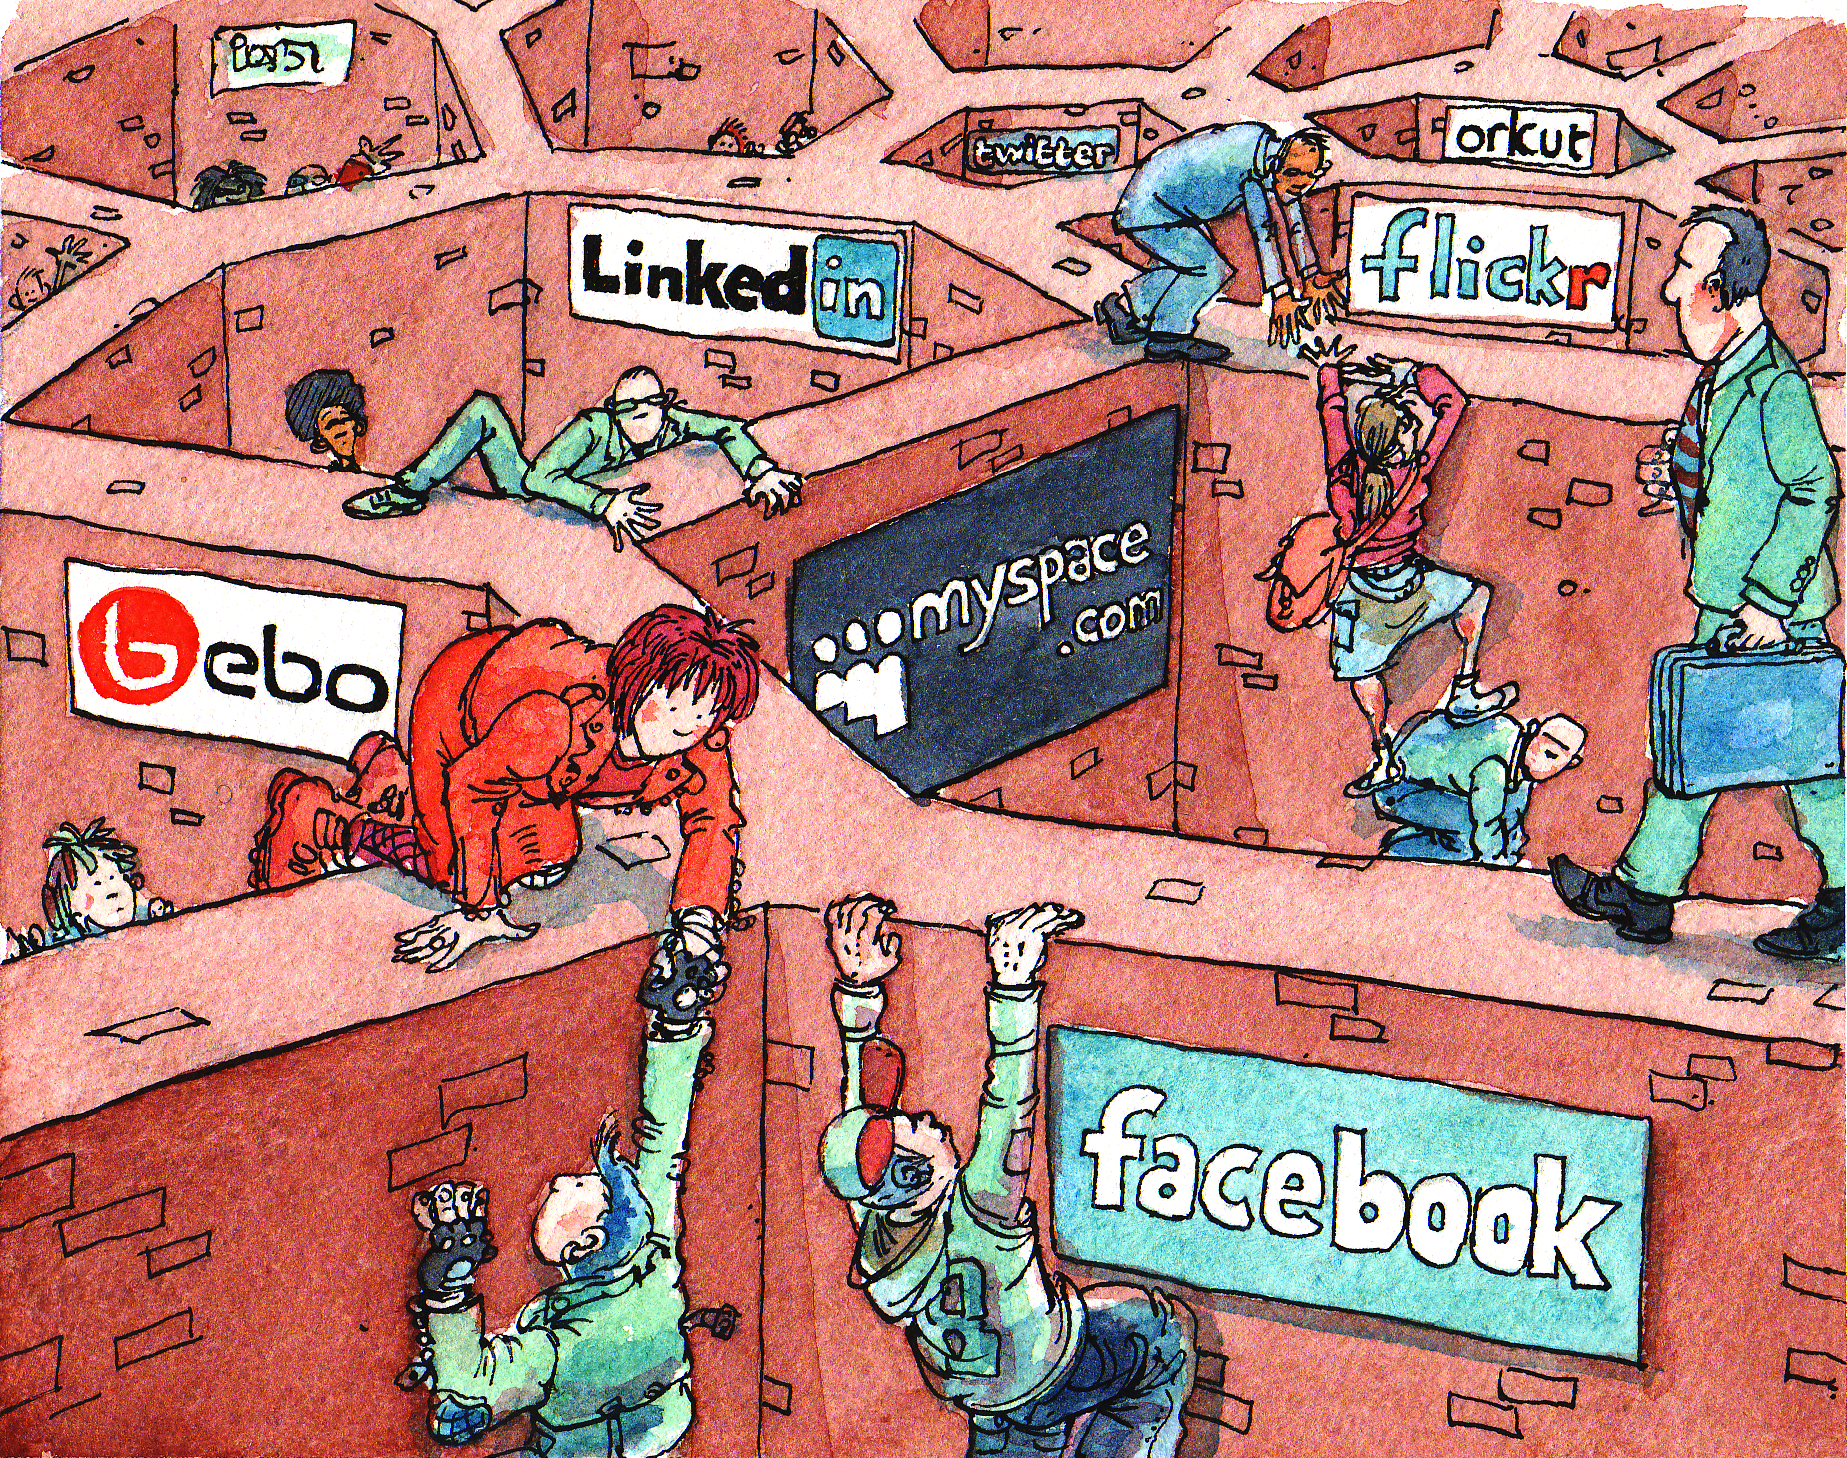
\includegraphics[width=1.0\linewidth]{./resources/davidsimonds.png}
\caption{Social networks as walled gardens.~\cite{DavidSimonds}}
\label{fig:DavidSimonds}
\end{figure}

%%%%%%%%%%% The bibliography starts:
\bibliographystyle{abbrv}
\bibliography{swj2012}

\end{document}